\mode*
\section{The idea}%
\label{TheIdea}

Alice is an activist who organizes a demonstration for some cause.
Her main goal after the protest is to provide verifiable data.
There are several problems:
\begin{itemize}
  \item Alice must prove that the data is related to the event, that it is not 
    reused data from previous protests.
  \item Alice must provide data which can be used for the desired verification.
  \item Alice must also consider the privacy of the participating individuals.
\end{itemize}

\begin{frame}<presentation>
  \begin{itemize}
    \item Alice must prove that the data is related to the event.
    \item Alice must provide data with verifiable properties.
    \item Alice must consider the privacy of the participants.
  \end{itemize}
\end{frame}

Since many of the current techniques are based on photos, we will give an 
example of Alice's problems in that setting.
How can she ensure that photos from a demonstration are authentic?
We can probably recognize the location that the photo is portraying, however, 
this might just as well be a reconstruction or entirely computer generated.
We cannot trust the meta-data of the photo, such as time-stamps of the file, 
because these can easily be manipulated.
So the only thing we can say for sure is that the photo was taken at the latest 
at the time of publication.
Now, if we cannot trust these photos, how can we determine the number of 
participants of a demonstration?
Furthermore, how can Alice protect the privacy of those in the photos?

%However, to complicate things further,
%\blockcquote{VenezuelanStateWorkersCalledToParticipate}{%
%  \textins*{m}any of Venezuela’s 2.8 million state workers have reported 
%  getting text messages, phone calls and being required to attend political 
%  rallies during work hours
%}.
%
%\blockcquote{BBConVenezuelaProtestBan}{%
%  Venezuela is banning protests that could "disturb or affect" Sunday's 
%  controversial election for a new constituent assembly.
%}
%
%\blockcquote{BBConVenezuelaProtestBan}{%
%  Prison terms of between five and 10 years could be imposed on those 
%  contravening the ban,
%}
%
%\blockcquote{VenezuelanGovtBansProtesting}{%
%  Venezuelans are planning to defy a government ban on public demonstrations 
%  and risk deadly repression with marches across the country to protest against 
%  a vote Sunday that opposition forces say will mark the end of democracy
%}

\subsection{Verification}%
\label{Verification}

We have an adversarial setting between Alice the activist and Eve the evil 
regime: Alice wants to show large support against Eve, Eve wants to show little
support for Alice.
In this case we have two options:
either we trust Alice or Eve, or we must verify their claims.
We aim for verifiable claims.

In general, protesting is very similar to voting: both are many individuals 
expressing their opinion.
These opinions can be sensitive, hence we desire to have similar properties of 
verification and privacy for participation in a protest as there is for voting.
In the context of (electronic) voting protocols, there are three requirements 
for verification~\cite{VerifyingPrivacyPropertiesOfVotingProtocols}:
\begin{frame}
\begin{requirements}[V]
\item\label{EligibilityVerif} Eligibility: anyone can verify that each vote 
  cast is legitimate.
\item\label{UniversalVerif} Universal verifiability: anyone can verify that the 
  result is according to the cast votes.
\item\label{IndividualVerif} Individual verifiability: every voter can verify 
  that their vote is included in the result.
\end{requirements}
\end{frame}
We can translate these to the case of participation in a demonstration, then 
each vote would be replaced by a proof of participation.

\Cref{EligibilityVerif} would in this case mean that anyone can verify that 
each participation proof belongs to a unique individual, i.e.\ to prevent Sybil 
attacks.
They must also be able to verify that each proof is indeed related to the 
event.
We must associate the proof to the event both spatially (the correct location) 
and temporally (it is related to the time-interval of the event).
We can essentially divide it into the following requirements:
\begin{requirements}[\ref*{EligibilityVerif}.]
  \item\label{CreatedAfterStart} Prove that the data was created after the 
    start of the event.
  \item\label{CreatedBeforeEnd} Prove that the data was created before the end 
    of the event.
  \item\label{SpatiallyRelated} Prove that the data is spatially related to the 
    physical location of the event.
  \item\label{CountOnce} Prove that no individual can be counted more than 
    once.
  \item\label{DesignatedEvent} Prove that the data is designated for the event.
\end{requirements}

\mode<presentation>{%
\begin{frame}
  \begin{requirements}[V\ref*{EligibilityVerif}.]
  \item\label{CreatedAfterStart} Prove that the data was created after the 
    start of the event.
  \item\label{CreatedBeforeEnd} Prove that the data was created before the end 
    of the event.
  \item\label{SpatiallyRelated} Prove that the data is spatially related to the 
    physical location of the event.
  \item\label{CountOnce} Prove that no individual can be counted more than 
    once.
  \item\label{DesignatedEvent} Prove that the data is designated for the event.
\end{requirements}
\end{frame}
}

\subsubsection{Temporal eligibility}

\Cref{CreatedBeforeEnd,CreatedAfterStart} requires a \emph{partially ordered 
  set}\footnote{%
  A relation \(\preceq\) which is reflexive, antisymmetric and transitive.
} of objects.
If some objects in the set relate to known points in time, then the partial 
order relates the data to the time of the event.
This allows us to \emph{verify the data temporally}.

One primitive that fulfils \cref{CreatedAfterStart,CreatedBeforeEnd} is a 
blockchain.
There are also other structures, e.g.\ a directed graph that 
converges~\cite{BlockchainFreeCryptocurrencies}.
(See \cref{PosetGraph}.)
For generality, we will use the terminology of 
\textcite{BlockchainFreeCryptocurrencies} and simply call this storage 
structure \iac{tposet}.

\begin{frame}
\begin{figure}
  \centering
  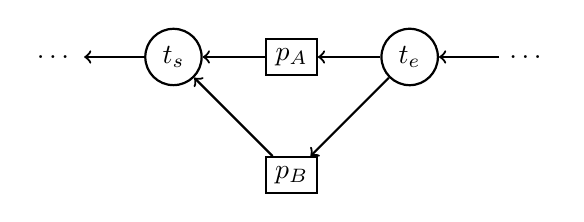
\begin{tikzpicture}[->,auto,node distance=1.5cm,thick,
  proof node/.style={rectangle,draw},
  time node/.style={circle,draw}]

  \node (prev) {\dots};
  \node[time node] (ts) [right of=prev] {$t_s$};
  \node[proof node] (pA) [right of=ts] {$p_A$};
  \node[proof node] (pB) [below of=pA] {$p_B$};
  \node[time node] (te) [right of=pA] {$t_e$};
  \node (succ) [right of=te] {\dots};

  \path
  (succ) edge node {} (te)
  (te) edge node {} (pB)
  (pB) edge node {} (ts)
  (te) edge node {} (pA)
  (pA) edge node {} (ts)
  (ts) edge node {} (prev);

\end{tikzpicture}

  \mode<article>{%
    \caption{%
      Alice submits proof \(p_A\) and Bob submits proof \(p_B\).
      We have \(t_s\prec p_A, p_B\prec t_e\), but \((p_A, p_B)\notin \prec\) 
      are incomparable.
    }\label{PosetGraph}
  }
\end{figure}

\mode<presentation>{%
  \only<1>{%
    \begin{idea}[Temporal eligibility]
      \begin{itemize}
        \item We need a partially ordered set (poset).

          \pause{}

        \item There is a mechanism that provides this property: a blockchain.
        \item There are also other structures, e.g.\ a directed 
          graph~\cite{BlockchainFreeCryptocurrencies}.
      \end{itemize}
    \end{idea}
  }
  \only<3>{%
    \begin{idea}[Created before end]
      \begin{itemize}
        \item Submit the proof to storage.
        \item The proof must've been created before it was included (duh!).
        \item If included before \(t_e\), then it was created before \(t_e\).
      \end{itemize}
    \end{idea}
  }
  \only<4>{%
    \begin{idea}[Created after start]
      \begin{itemize}
        \item Include an unpredictable value in the proof.
        \item This could be e.g.\ the hash of the \enquote{head} of the 
          \ac{tposet}, (\(t_s\) in the figure).
        \item This prevents creating proofs for future protests.
      \end{itemize}
    \end{idea}
  }
}
\end{frame}

\Cref{CreatedBeforeEnd} is straight-forward, Alice and Bob simply add their 
proofs to the \ac{tposet} \emph{in (time-wise) relation to the event}.
In \cref{PosetGraph}, if \(t_e\) is verifiably related to the end of the 
protest, then the relation will guarantee that \(p_A, p_B\) were created before 
the end of the protest.
Then we know that they cannot have been created after the event.

For \cref{CreatedAfterStart} Alice and Bob must include an unpredictable value 
in their proofs, e.g.\ \(t_s\) in \cref{PosetGraph}.
This means that if \(t_s\) is sufficiently close (time-wise) to the protest and 
has sufficiently high entropy, then Alice or Bob cannot create a proof and keep 
it for a future protest.

They can use an older value (pick one from the history of the \ac{tposet}) when 
they create their proofs.
This will only expand the interval of possible creation into the past.
This will not help their cause, as anyone will recognize that the proof could 
be created at any time in that interval, i.e.\ possibly before the protest.

\begin{question}
  How hard is it to reuse old proofs?
  Forge all signatures due to changed values?
\end{question}

\subsubsection{Spatial eligibility}

\Cref{SpatiallyRelated} binds the data spatially to the location, which allows 
us to \emph{verify the data spatially}.

If we include \iac{LP}, this will tie the proof to the physical location and, 
thus, solve \cref{SpatiallyRelated}.
The \ac{LP} is \enquote{witnessed} (signed) by other participants.
The \ac{LP} contains coarse coordinates of the location, which must be within 
the protest area to be valid.
This allows Bob the protester to move within the protest area to collect 
witnesses (signatures).
It also provides privacy since the location cannot be used to deanonymize Bob's 
proof --- e.g.\ to correlate the location in his proof with captured 
surveillance footage.

\mode<presentation>{%
\begin{frame}
  \begin{figure}
    \centering
    \begin{tikzpicture}
      \tikzset{grow'=right,level distance=5em}
      \Tree [.Proof
      [.{wsig} {\(x,y\)} {$t_s$} ]
      {\dots}
      [.{wsig} {\dots} ]
      ]
    \end{tikzpicture}
  \end{figure}

  \begin{idea}[Spatial eligibility]
    \begin{itemize}
      \item Include \iac{LP} which is \enquote{witnessed} (signed) by other 
        participants.
      \item We have a coarse location, just within the protest area.
      \item This allows protesters to move around to collect signatures.
      \item This provides privacy for the location, e.g.\ cannot map to 
        surveillance cameras.
    \end{itemize}
  \end{idea}
\end{frame}
}

\begin{question}
  Why should anyone trust these witnesses?
  What are the assumptions?
  Signed over a short period of time?\footnote{%
    In a sense, if they collude they have shown support for the cause.
    As long as they are not Sybil it should be fine?
  }
\end{question}

\mode<none>{%
\begin{frame}
  \begin{idea}[Transitive trust]
    \begin{itemize}
      \item Trusted journalist Jane attends to report.
      \item She witnesses Alice's proof.

        \pause{}

      \item Alice witnesses Bob's proof.
      \item Alice's (secret key's) transportation is physically limited.
      \item Trust on Bob's proof is proportional to time from when Jane 
        witnessed Alice's proof.
    \end{itemize}
  \end{idea}
\end{frame}

\begin{frame}
  \begin{figure}
    \centering
    \begin{tikzpicture}
      \tikzset{grow'=right,level distance=5em}
      \Tree [.Proof
      [.{wsig} {\(x,y\)} {$t_s$} [.{\color{red}tsig} {$t_s'$} ] ]
      {\dots}
      [.{wsig} {\dots} ]
      ]
    \end{tikzpicture}
  \end{figure}

  \begin{remark}
    \begin{itemize}
      \item Secret key in hardware.
      \item Alice's witness signature must depend on Jane's.
      \item High-precision relation to time?
    \end{itemize}
  \end{remark}
\end{frame}
}

We will introduce a notion of transitivity for trust in these proofs.
The \emph{trusted} journalist Jane attends the protest to report on it.
She witnesses some participants' \acp{LP}, say Alice's \ac{LP} for example.
Now Alice's \ac{LP} can be trusted as correct at that point in time.
Alice's ability to travel is physically limited.
Thus a verifier can trust any \ac{LP} that Alice witnesses proportionally to 
the time that has passed since Jane witnessed Alice's \ac{LP}.
We can apply this argument recursively for any other participant's \ac{LP} that 
Alice has witnessed.
However, this requires some assumptions:
\begin{itemize}
  \item It is actually Alice's signing key must have physically limited travel.
    This can be assumed for signing keys that are embedded into hardware by 
    some trusted person.
  \item Alice's witness signature must depend on Jane's witness signature, to 
    prove that Alice signed after Jane.
\end{itemize}
\begin{remark}
  This probably requires high-precision timestamps, i.e.\ a trusted 
  time-stamping server must be available during the protest.
  Or the proofs must be submitted to the \ac{tposet} during the protest.
\end{remark}

\begin{question}
  Trusted party for the group signatures?
\end{question}
\begin{question}
  How can we do \acp{LP} with 1000s of witnesses each?
  Can we do some preprocessing?
  Ad-hoc networks, broadcast \acp{LP}?
\end{question}
\begin{question}
  Must tie credentials to something unique: phone, phone subscription?
  Cannot register twice, government control?
\end{question}

\begin{question}
  What if Alice acts as a witness for Eve's agents?
  Can that violate her privacy?
\end{question}
\begin{question}
  What if Eve's agents act as witnesses?
  Can they track their signatures to track users?
  Can Alice detect if this happens?
\end{question}

\subsubsection{Linkability and designated protest}

\Cref{CountOnce} is required to prevent Sybil attacks, i.e.\ that one 
individual can provide two proofs of participation and thus be counted twice.
That situation should be detectable.
We can do this by ensuring that Alice cannot produce two valid proofs which
are unlinkable.
This can be done by including a signature made by a verified key.
(We will discuss the privacy aspects in \cref{Privacy}.)

\Cref{DesignatedEvent} focuses on the problem that there might be a counter 
protest at the same time and place, these would have the same spatial and 
temporal properties.
To distinguish them, we also need to prove for which of these events that a 
proof is designated.
This can be achieved by a unique identifier for a protest, e.g.\ the hash of 
its \enquote{manifesto}.

\begin{frame}
\begin{figure}
  \centering
  \mode<presentation>{%
    \only<1>{%
      \begin{tikzpicture}
        \tikzset{grow'=right,level distance=5em}
        \Tree [.Proof
        [.{wsig} {\(x,y\)} {$t_s$} [.{\color{red}osig} {$t_s'$} ]
        %[.tsig {$t_s''$} ]
        ]
        {\dots}
        [.{wsig} {\dots} ]
        ]
      \end{tikzpicture}
    }
  }
  \only<2>{%
    \begin{tikzpicture}
      \tikzset{grow'=right,level distance=5em}
      \Tree [.Proof
      [.{wsig} {\(x,y\)} {$t_s$} [.{osig} 
      [.{\mode<presentation>{\color{red}}\(id\)} manifesto ] {$t_s'$} ]
      %[.tsig {$t_s''$} ]
      ]
      {\dots}
      [.{wsig} {\dots} ]
      ]
    \end{tikzpicture}
  }
  \mode<article>{%
    \caption{%
      The proof depends on several witness signatures (wsig), each of which 
      depends on the owner's signature (osig), which depends on the \(id\) of the
      protest and the head of the \ac{tposet}.
      Whenever possible, the witness signature should include proof that the 
      witness themself has been witnessed by a trusted witness (tsig).
    }
  }
\end{figure}

\mode<presentation>{%
  \only<1>{%
    \begin{idea}[Count once]
      \begin{itemize}
        \item Any two proofs by the same individual are linkable.
        \item Includes signature made by a verified key.
      \end{itemize}
    \end{idea}
  }

  \only<2>{%
    \begin{idea}[Designated event]
      \begin{itemize}
        \item Include a protest-specific identifier.
        \item E.g.\ hash of the \enquote{manifesto}.
      \end{itemize}
    \end{idea}
  }
}
\end{frame}

\subsubsection{Individual and universal verifiability}

If the proofs are stored publicly, then an individual can check that their 
proof has been included (committed) there.
Thus \cref{IndividualVerif} is fulfilled.
Similarly for universal verifiability.
If the storage is public, then anyone can download all the proofs, verify their 
eligibility and count them.
Thus anyone can verify the result, which fulfils \cref{UniversalVerif}.
To have any verifiability, we need the storage to be immutable --- i.e.\ it 
prevents malicious changes.

\mode<presentation>{%
\begin{frame}
  \begin{idea}[Individual verifiability]
    \begin{itemize}
      \item Proofs are stored (committed) publicly.
      \item Each participant can check that their proof is indeed included.
    \end{itemize}
  \end{idea}

  \pause{}

  \begin{idea}[Universal verifiability]
    \begin{itemize}
      \item Proofs are stored (committed) publicly.
      \item Anyone can download all proofs, verify eligibility and then count 
        them.
    \end{itemize}
  \end{idea}
\end{frame}
}

\subsection{Privacy}%
\label{Privacy}

We also need privacy in addition to the verification requirements.
As we indirectly pointed out earlier, we focus on the privacy provided to Alice 
and Bob by the data.
So as long as Alice and Bob can conceal their identities at the demonstration 
and escape without arrest, their support is recorded in the data while their 
privacy is not violated.
(Following this line of thinking, it can actually be beneficial for the privacy 
of the demonstrators to mix with the participants of any counter-demonstrations 
--- since the counts will still be correct.)

In voting, we have the following requirements:
\begin{frame}
\begin{requirements}[P]
\item\label{VotePrivacy} Vote privacy: the voting does not reveal any 
  individual vote.
\item\label{ReceiptFreeness} Receipt freeness: the voting system does not 
  provide any data that can be used as a proof of how the voter voted.
\item\label{CoercionResistance} Coercion resistance: a voter cannot cooperate 
  with a coercer to prove the vote was cast in any particular way.
\end{requirements}
\pause{}
\mode<presentation>{%
  \begin{remark}
    P\ref{CoercionResistance} \(\implies\)
    P\ref{ReceiptFreeness} \(\implies\)
    P\ref{VotePrivacy}
  \end{remark}
}
\end{frame}
\Textcite{VerifyingPrivacyPropertiesOfVotingProtocols} showed that 
\cref{CoercionResistance} implies \cref{ReceiptFreeness}, which in turn implies
\cref{VotePrivacy}.
\Cref{CoercionResistance} is probably not possible to achieve for protests:
e.g.\ Eve can simply physically bring Alice to a protest against her will.
This leaves us with \cref{ReceiptFreeness,VotePrivacy}.

\mode<none>{%
\begin{frame}
  \begin{remark}
    \begin{itemize}
      \item Coercion resistance is difficult to achieve for voting.
      \item It doesn't make much sense for protests.
      \item E.g.\ Eve physically brings Alice to a protest she doesn't want to 
        participate in.
      \item That leaves us with receipt freeness and vote privacy.
    \end{itemize}
  \end{remark}
\end{frame}
}

\subsubsection{Participation-proof privacy}

A demonstration is very different from voting in one sense: at a demonstration, 
Alice must be physically present and that very presence shows her support for 
the cause.
In voting, on the other hand, everyone is present and Alice has multiple 
options which are not revealed by her mere presence.
% XXX Check if unlinkable is the correct term
Hence, if Alice submits a proof of participation, the proof must be unlinkable 
to Alice, yet, if Alice submits another proof, those two proofs must be 
linkable (due to eligibility verification, \cref{EligibilityVerif}) so that 
Alice is not counted twice.
This is fine, since we do not want to catch any cheater, we just do not want to
count them more than once.

\mode<presentation>{%
\begin{frame}
  \begin{remark}
    \begin{itemize}
      \item Voting: different alternatives when participating.
      \item Protesting: participation implies the alternative.
    \end{itemize}
  \end{remark}

  \pause{}

  \begin{idea}[Proof privacy]
    \begin{itemize}
      \item Eve shouldn't be able to link Alice's published proof back to 
        Alice.
      \item But if Alice publishes two proofs, those two are linkable.
      \item We're not interested in unmasking trolls, just not count them more 
        than once.
    \end{itemize}
  \end{idea}
\end{frame}
}

\begin{frame}
  \begin{remark}
    Unique ring signatures~\cite{UniqueRingSignatures} has this property: two 
    signatures are linked with high probability.
  \end{remark}

  \begin{question}
    Can we link a verified key to a unique ring signature key?
  \end{question}

  \pause{}

  \begin{question}
    How to submit the proofs to the system?
  \end{question}
\end{frame}

\subsubsection{Receipt freeness}

Receipt freeness implies that Alice enjoys deniability against Eve:
Eve should not be able to use the published proof to tie it to Alice, even if 
Eve has access to Alice's device (i.e.\ all her private keys).
E.g.\ Eve should not be able to reproduce the same proof and thus verify that 
Alice has created one of the proofs.

\mode<presentation>{%
\begin{frame}
  \begin{remark}
    The proof itself is a sort of receipt.
  \end{remark}

  \pause{}

  \begin{idea}[Receipt freeness (deniability)]
    \begin{itemize}
      \item Alice submits her proof.
      \item She stores the hash of the head of the \ac{tposet}.
      \item She removes the proof and signature key.
    \end{itemize}
  \end{idea}
\end{frame}
}

\begin{frame}
\mode<presentation>{%
  \begin{idea}
    \begin{itemize}
      \item If Eve compromises Alice's device, she should not be able to use it 
        to verify that she participated.

      \item We need a signature scheme that cannot reproduce the same signature 
        when run on the same inputs.

      \item E.g.\ a short-term and a long-term credential, then Alice can 
        drop the short-term credential.

      \item But Alice should still not be able to participate twice.
    \end{itemize}
  \end{idea}
}

  \pause{}

  \begin{question}
    Is there such a signature scheme?
    Can we construct it?
  \end{question}
\end{frame}

Say that Alice submits her proof and stores the hash of the head of the 
\ac{tposet} after her proof is included.
Now she can remove her proof and just keep the hash to verify that her proof is 
still there.
She can also remove her signature key, so that Eve cannot use it to reproduce 
the signature using the same inputs.

\subsubsection{Architecture}

We also have an architectural problem.
If the system is only run by volunteering activists, then Eve can simply 
analyse network traffic and look for people running nodes in the system.

\begin{question}
  Shall we offer a platform that is run by a variety of institutions who 
  offers to verify protests?
  Or go strictly peer-to-peer?
\end{question}

\begin{question}
  If strictly peer-to-peer, and only run by protesters, one can infer that 
  they are protesters by running such a node.
  Can this be mitigated?
\end{question}

Similarly, we have the problem of how protesters submit their proofs to the 
system.
This must be done anonymously.
Otherwise Eve can analyse the network traffic to find out who submitted proofs 
to the system.
The main problem here is that the participants must be indistinguishable from 
non-participants.
This means that we cannot use special-purpose anonymizing 
technologies.

\begin{question}
  How do we submit the proofs to storage?
  Voting normally uses mix-nets (provable shuffles).
\end{question}

\begin{remark}
  We must mix participants with non-participants.
\end{remark}

